\chapter{麻雀ゲーム理論}
\label{chap:relevantstudy}

本章では麻雀のゲーム理論的な位置づけと、AIを作る上で課題となる点を述べる。また、麻雀の一般論や関連研究についても同様に述べる。

\section{麻雀のゲーム理論的分類}
昨今では、Googleが囲碁の世界で世界チャンピオンを破ったことは記憶に新しく\cite{go}、あらゆるゲームAIが様々な分野で活躍している。二人零和有限確定完全情報ゲームに分類されるチェス、将棋、オセロ、囲碁などは既にトップレベルの実力を達成している。これらのゲームはまず、二人零和ゲームであるために、自分の得点と相手の得点の関係性が明確である。自分の得点はすなわち相手の失点と等価であり、また、自分の失点は相手の失点と等価である。そのため、自分を有利な立場にするような戦略のモデルが作りやすく、これらの研究はいい結果を残している。また、有限であることも重要である。ゲームが有限な手数で終わるということがわかっている場合、モンテカルロ法によるシミュレーションなどで最終スコアから手の良さを逆算することが可能であるからである。これが無限になるケースだと、探索範囲が無限に広がるどころか、ゲーム終了時のスコアを取れない場合があるので難しい。さらに、確定完全情報ゲームであることは、ゲームの複雑性を少なくすることにおいて大切である。手の選択によって得られる結果が確定でないゲームでは、特定の手によって起こる結果をモデル化すること自体研究対象となる。また、不完全情報ゲームでは、相手プレイヤーや場のモデルも構成しないといけないため、同様に複雑性を増す。ゲーム理論的分類によるそれぞれの特徴を表\ref{game}に示す。


\begin{table}[H]
  \caption{ゲーム理論的分類}
  \label{game}
  \begin{center}
  \begin{tabular}{c|p{5.75cm}|p{6.25cm}}
    \hline
    分類 & 二人零和有限確定完全情報ゲーム &  四人零和有限不確定不完全情報ゲーム \\\hline\hline
    対象 & チェス・将棋・オセロなど & 麻雀 \\\hline
    プレイ人数  & 2人 & 4人 \\\hline
    得点の関係 & プレイヤーの得点の合計は常に一定 & プレイヤーの得点の合計は常に一定 \\\hline
    終了条件 & ランダムに手を選択している場合でも理論上いずれ必ず終了する & ランダムに手を選択している場合でも理論上いずれ必ず終了する\\\hline
    選択による結果 & 特定の手によって得られる結果は常に同じ & 特定の手によって得られる結果が異なる場合がある\\\hline
    情報 & 相手プレイヤーの選択と場に起きている事象を全て知ることができる & 相手プレイヤーの選択と場に起きている事象を全ては知ることができない\\\hline
  \end{tabular}\end{center}
\end{table}


本研究の対象となる麻雀は、分類するとしたならば、四人零和有限不確定不完全情報ゲームである。以上に述べたような二人零和有限確定完全情報ゲームと異なり、課題が多いために麻雀のAIは未だにトッププレイヤーレベルの実力に達しているものは存在しない。

まず際立つ問題がプレイヤーが4人という多人数であることである。2人プレイヤーでは自分の得点と相手の失点は等価であったが、4人プレイヤーの場合自分と特定の相手プレイヤーの得点の関係は同様ではない。すなわち、プレイヤーごとに達成すべき目的が異なる場合が存在するため、単純なモデルを作ることが難しい。この多人数性の問題を解決するには、プレイヤーを1人とした1人麻雀の利用が考えられる。これは、麻雀プレイヤーが自分の実力を高めるために練習として使う用途があったが、水上ら\cite{bakuuti2013}などが麻雀の研究をする際に使用している。本研究でも、評価としてこの1人麻雀を利用する。

次に、不確定性が存在する面も、麻雀のAIを作る際に難しい問題となっている。選択した手によって得られる結果が確定でない以上、これらは確率的にしか求めることが出来ない。この問題に対してのアプローチとしては、途中局面のヒューリスティクスを用いて手の優劣を決定する手法の他に、モンテカルロ法によるシミュレーションを用いた方法などが挙げられる。本研究では前者を対象とするが、これらの関連研究については次節以降に解説する。

% プレイ人数に着目した研究としてはポーカーを用いたもの \cite{poker},\cite{hurui} がある。これらの手法では 2 プレイヤでのゲームを強くしてから多人数に適応する方法がとられている。ポーカーは2 プレイヤであればナッシュ均衡戦略を用いることで世界チャンピオンに勝っているが、ポーカーは 2人から 10 人程度で参加可能なゲームであり人数が増える
% と状態数が指数関数的に増大するためナッシュ均衡戦略の計算は難しい。そこで 2 人で行われたナッシュ均衡戦略を3 人限定で拡張する方法、プレイヤの行動を削減、抽象化することでより少ない人数の少ないゲームを想定する方法がとられた。

\section{麻雀の一般論}
この節では麻雀の一般論について述べる。前節で述べたように、麻雀は多人数性と不完全情報の観点から、複雑さを極めるルールとなっている。ただし、戦略について大きく分けると、自分の得点を加算する攻めの技術と、失点を防ぐための守りの技術に分類することができる。これについてこの節では解説する。また、本研究では攻めについて取り扱うため、攻めの戦略において重要である指標についても説明する。
\subsection{押しと降り}
一般に、麻雀において攻める技術を押し、守る技術のことを降りという。麻雀で得点を加算することは、原則自分の手を和了ることによってのみ実現される。したがって、押しの技術に関してはまず自分の手を和了まで持っていけるかということが重要となる。和了の形式としてはツモ和了とロン和了が存在し、ツモ和了では他の相手プレイヤー全てから得点を奪い、ロン和了では上がり牌を河に捨てたプレイヤーから得点を奪う。次の優先度として、和了の形、すなわち役によって加算される際の得点が異なるため、できるだけ高い打点の構成で上がることが求められる。

一方、麻雀で失点となる局面は、原則相手プレイヤーが和了した時である。失点の方式は2つあり、放銃失点と被ツモ失点によるものである。前述した相手プレイヤーがロン和了となるような牌を自分が河に捨ててしまった場合は放銃失点となり、相手プレイヤーがツモ和了した場合は被ツモ失点として得点を支払う。ただし、被ツモ失点の場合は他プレイヤーとともに失点を痛み分けすることになるので、放銃失点よりは失う得点が少ない。したがって、被ツモ失点は免れることは難しいが、放銃失点は自分の捨てる牌に注意することで免れることが可能となるため、降りの戦略としては主に相手プレイヤーをロン和了させないように打つことが基本となる。

\subsection{シャンテン数}
和了形は役によって多少の違いはあるが、一般に雀頭1つとメンツ4つで構成される。この形を、与えられた13牌の配牌から始め、山から1枚ツモり自分の手牌から1枚切る動作を繰り返すことで完成させることが和了となる。ここで、まだ和了形に至っていない牌姿において、和了までどれだけの距離があるかを示すための指標としてシャンテン数が存在する。シャンテン数とは、実際には和了形ではなくその一つ手前の状況である聴牌を基準としたものであるが、基準としては和了までの距離として使って構わない。シャンテン数の具体的な定義は、現在の牌姿から最短何回のツモで聴牌にたどり着くことができるかをである。具体例を図\ref{2syanten}に示す。この場合は、最短であと3つの必要な牌をツモることで和了することができ、あと2つの必要な牌をツモることで聴牌であるため、この牌姿は2シャンテンである。

\begin{figure}[H]
 \centering
 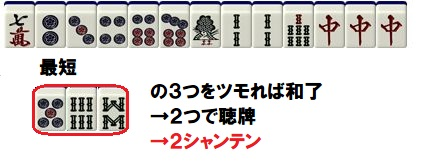
\includegraphics[keepaspectratio, scale=1,bb=0 0 320 200]
      {img/2syanten.jpg}
 \caption{シャンテン数}
 \label{2syanten}
\end{figure}

\section{関連研究}
和了率を高めるための研究としては、大きく分けると以下のようになる。

\begin{itemize}
 \item {\bf モンテカルロ法によるシミュレーションを用いた方法} \mbox{}\\ 
 	麻雀は不確定不完全情報ゲームであるものの、その手数は有限である。したがって、開局時からランダムな手を選択し続けてもいずれ必ず終局となる。麻雀におけるモンテカルロ法とは、このようにランダムな手を選択し続けて終局までプレイする(これを以下プレイアウトと呼ぶ)ことを繰り返す方法である。特定の手を選択した後にプレイアウトを複数回行い、そのゲーム結果を平均してその手の良さとする。
 \item {\bf 上級者の牌譜を学習してモデルを作る方法} \mbox{}\\
 	麻雀は多人数性要素、不確定要素、不完全情報要素によって、総合的な要素を兼ね備えたモデルを一から作り上げることは非常に難しい。そのため、上級者の試合データを利用し、複数の特徴量によってその打ち筋を学習し、上級者のプレイとの一致率を高めるようなモデルを制作する方法である。
 \item {\bf 途中局面のヒューリスティクスを用いた方法} \mbox{}\\ 
 	先に述べたように、麻雀の途中局面の優劣を、総合的に比較する指標を作ることは極めて難しい。しかし、部分的であれば利用できる指標は存在する。例えば和了率においては、ある牌姿におけるシャンテン数、有効牌の数などがそれに当たる。これらの指標を利用し、ヒューリスティクス的に最適な手を選ぶようにする方法である。
\end{itemize}

上級者の牌譜を学習してモデルを作る方法では北川ら\cite{kitakawa}や水上ら\cite{bakuuti2013}の研究が報告されているが、いずれも面前においての和了率は平均プレイヤの実力に至っていない。これらは、4人麻雀の牌譜を使っていることで、4人麻雀独特の打ち方を排除できない問題や、上級者が認知できない最適解を求められない問題があった。

また、モンテカルロ法によるシミュレーションを用いた方法では、麻雀は分岐が多すぎるため探索範囲が広く、そのまま適用しても精度が出ない。したがってこの分野の研究としては、探索範囲を限定することができるUCB\cite{UCB}やUCT\cite{UCT}と言った手法が利用されている。UCBを利用した打牌アルゴリズムとしては中張らの研究が\cite{LinUCB_mahjong}あげられる。また、UCTを利用した打牌アルゴリズムでは、三木らの研究が\cite{miki}挙げられる。これらはそれぞれの手法によって探索範囲を限定したシミュレーションを行っているが、麻雀の分岐局面が多すぎる問題に対してまだ課題が多く、平均プレイヤーを超える和了率は出せていない。

最後に途中局面のヒューリスティクスを用いた方法だが、面前の和了率を上げるためにはいい成績が出ている。この分野での研究としては、佐藤らの有効牌を数え上げることによって打牌するアルゴリズム\cite{zentsu}などがあげられる。相手プレイヤーに関する鳴きや打点などを考慮した観点からは劣る部分も多いが、面前の和了率については良い結果を残している。これらの研究は、本研究の手法と近いため、詳しく次章でまた解説する。

\subsection{水上らの研究}
水上らは、オンライン麻雀「天鳳」\cite{tenhou}の上級者のプレイヤーの牌譜データを学習し、平均化パーセプトロンを利用することで1人麻雀における和了率を高めた。以下平均化パーセプトロンについて述べる。

平均化パーセプトロンによるそれぞれの局面の評価式$f$は、特徴ベクトルを$x$、 重みベクトルを$w$とすると、式\ref{per1}と表される。

\begin{equation}
\label{per1}
\Large f(x,w) = \sum_{i=1}^{n} x_iw_i
\end{equation}

ツモった状態の手牌から、14枚の全ての牌をそれぞれ切った場合に対して、それらの上記の評価値を求める。次に上級者が牌譜で実際に行った打牌 $t0$ と評価値の最も高かった打牌 $t1$ を比較する。これらが一致しなかった場合、重みベクトルを式\ref{per2}を利用し更新する。

\begin{equation}
\label{per2}
\Large  w′ = w + x_{t0} − x_{t1}
\end{equation}

このようにして、平均化パーセプトロンにおける更新は行われる。全ての牌譜の局面に対しこれを繰り返し行い、毎局面の重みベクトルの平均値を最終的な重みとする。

これを利用した結果、水上らの1人麻雀プレイヤーの実力は平均プレイヤーを統計的に優位なレベルで超えることが出来た。しかし、4人麻雀の牌譜を元に使っていることによる1人麻雀とのズレや、上級者でも間違えやすい部分についての対策が打てない問題があった。そのため、1人麻雀の和了率は上級者には届かなかった。


\subsection{UCBを用いた研究}
通常のモンテカルロ探索では、ノードごとに期待される手の良さを途中で判定していないため、全てのノードに対して同じ回数のプレイアウトを行うことになる。(図\ref{d_monte})したがって、良い手が期待できないノードに対しても多くのプレイアウトを割り当てることになり、無駄なシミュレーションを行ってしまう事が考えられる。また、ノードによっては手の良さを決定する分岐がプレイアウトに対して大量にある場合、他のノードと同じ回数のプレイアウトでは十分な評価が出来ない可能性もある。このような問題に対しての解決手法として、Upper Confidence Bound (UCB) \cite{UCB}を用いたものが存在する。

\begin{figure}[h]
 \centering
 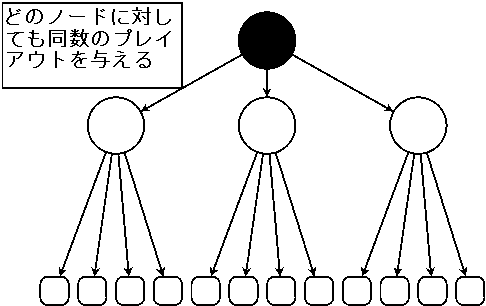
\includegraphics[keepaspectratio, scale=0.7,bb=0 0 330 260]
      {img/monte.png}
 \caption{通常のモンテカルロ探索}
 \label{d_monte}
\end{figure}

UCBの考え方を扱う方法では、一般にUCB1値が使われている。UCB1値を用いることによって各ノードの有望さをその都度確認し、全体のプレイアウトの回数や特定のノードで行われたプレイアウトの回数を考慮して、プレイアウトをどのノードに数多く割り当てるかということを判別することができる。
UCB1値は、子ノード$j$の平均報酬を${x_{j}}$、定数として$α$,親ノードの探索回数を$n$,子ノード$j$の探索回数を${n_{j}}$とした時、式\ref{UCB1value}で表される。

\begin{equation}
\label{UCB1value}
\Large UCB1 = \overline {x_{j}}+\alpha \sqrt {\displaystyle \frac {2\log{n}} {n_{j}}}
\end{equation}

通常のモンテカルロ探索では平均報酬を、そのまま全てのプレイアウトが終了するまで行った上で算出される平均値としていた。すなわち、上記の式では${x_{j}}$に当たるものである。しかし、UCB1ではこれに対し$\alpha \sqrt {\frac {2\log{n}} {n_{j}}}$で表される信頼度を加える。そうすることで、全てのプレイアウトを行うよりも前に信頼できる範囲を推定できる。これを利用し、多くのプレイアウトを割り当てなくとも、そのノードが有望かどうかを判別することが可能になる。(図\ref{ucb_monte})

\begin{figure}[h]
 \centering
 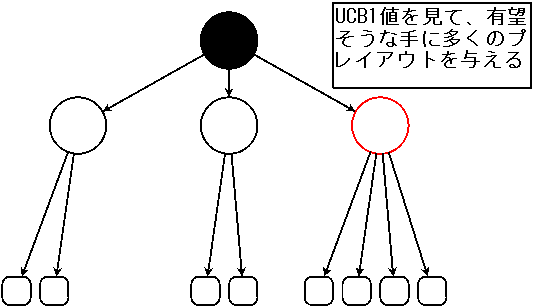
\includegraphics[keepaspectratio, scale=0.7,bb=0 0 330 260]
      {img/monteUCB.png}
 \caption{UCBを用いたモンテカルロ探索}
 \label{ucb_monte}
\end{figure}


このUCBを麻雀について適用した例は、中張ら\cite{LinUCB_mahjong}が報告している。中張らは、UCBを拡張した事前の学習を用いたLinUCBについてもその性能を評価している。しかし、1人麻雀の和了率を評価した結果では、和了率はどのアルゴリズムにおいても平均プレイヤーに10%以上の差をつけて劣っていた。UCBよりも性能が高いことが期待されていたLinUCBについても、良い特徴量を設計できずUCBよりも低い性能となった。したがってこの方法では、状況を劇的に改善する特徴量の設計などを発見しない限り、10%以上の和了率の向上は難しいと考えられる。

% \subsection{UCTを用いた研究}


